\chapter{Problem definition and the Proposed solution}

\section{3D Laser Line Scanners}


3D laser line scanners work on the principle of laser triangulation and use a camera chip in the receive path. The setup shown in Figure \ref{fig:laser_line_setup} consists of a camera sensor with an angle $\alpha$ from the vertical line, and a laser line source directed on top of the object. When the laser is cast onto the object, the laser line is captured by the camera sensor.


\begin{figure}[h]
    \centering
    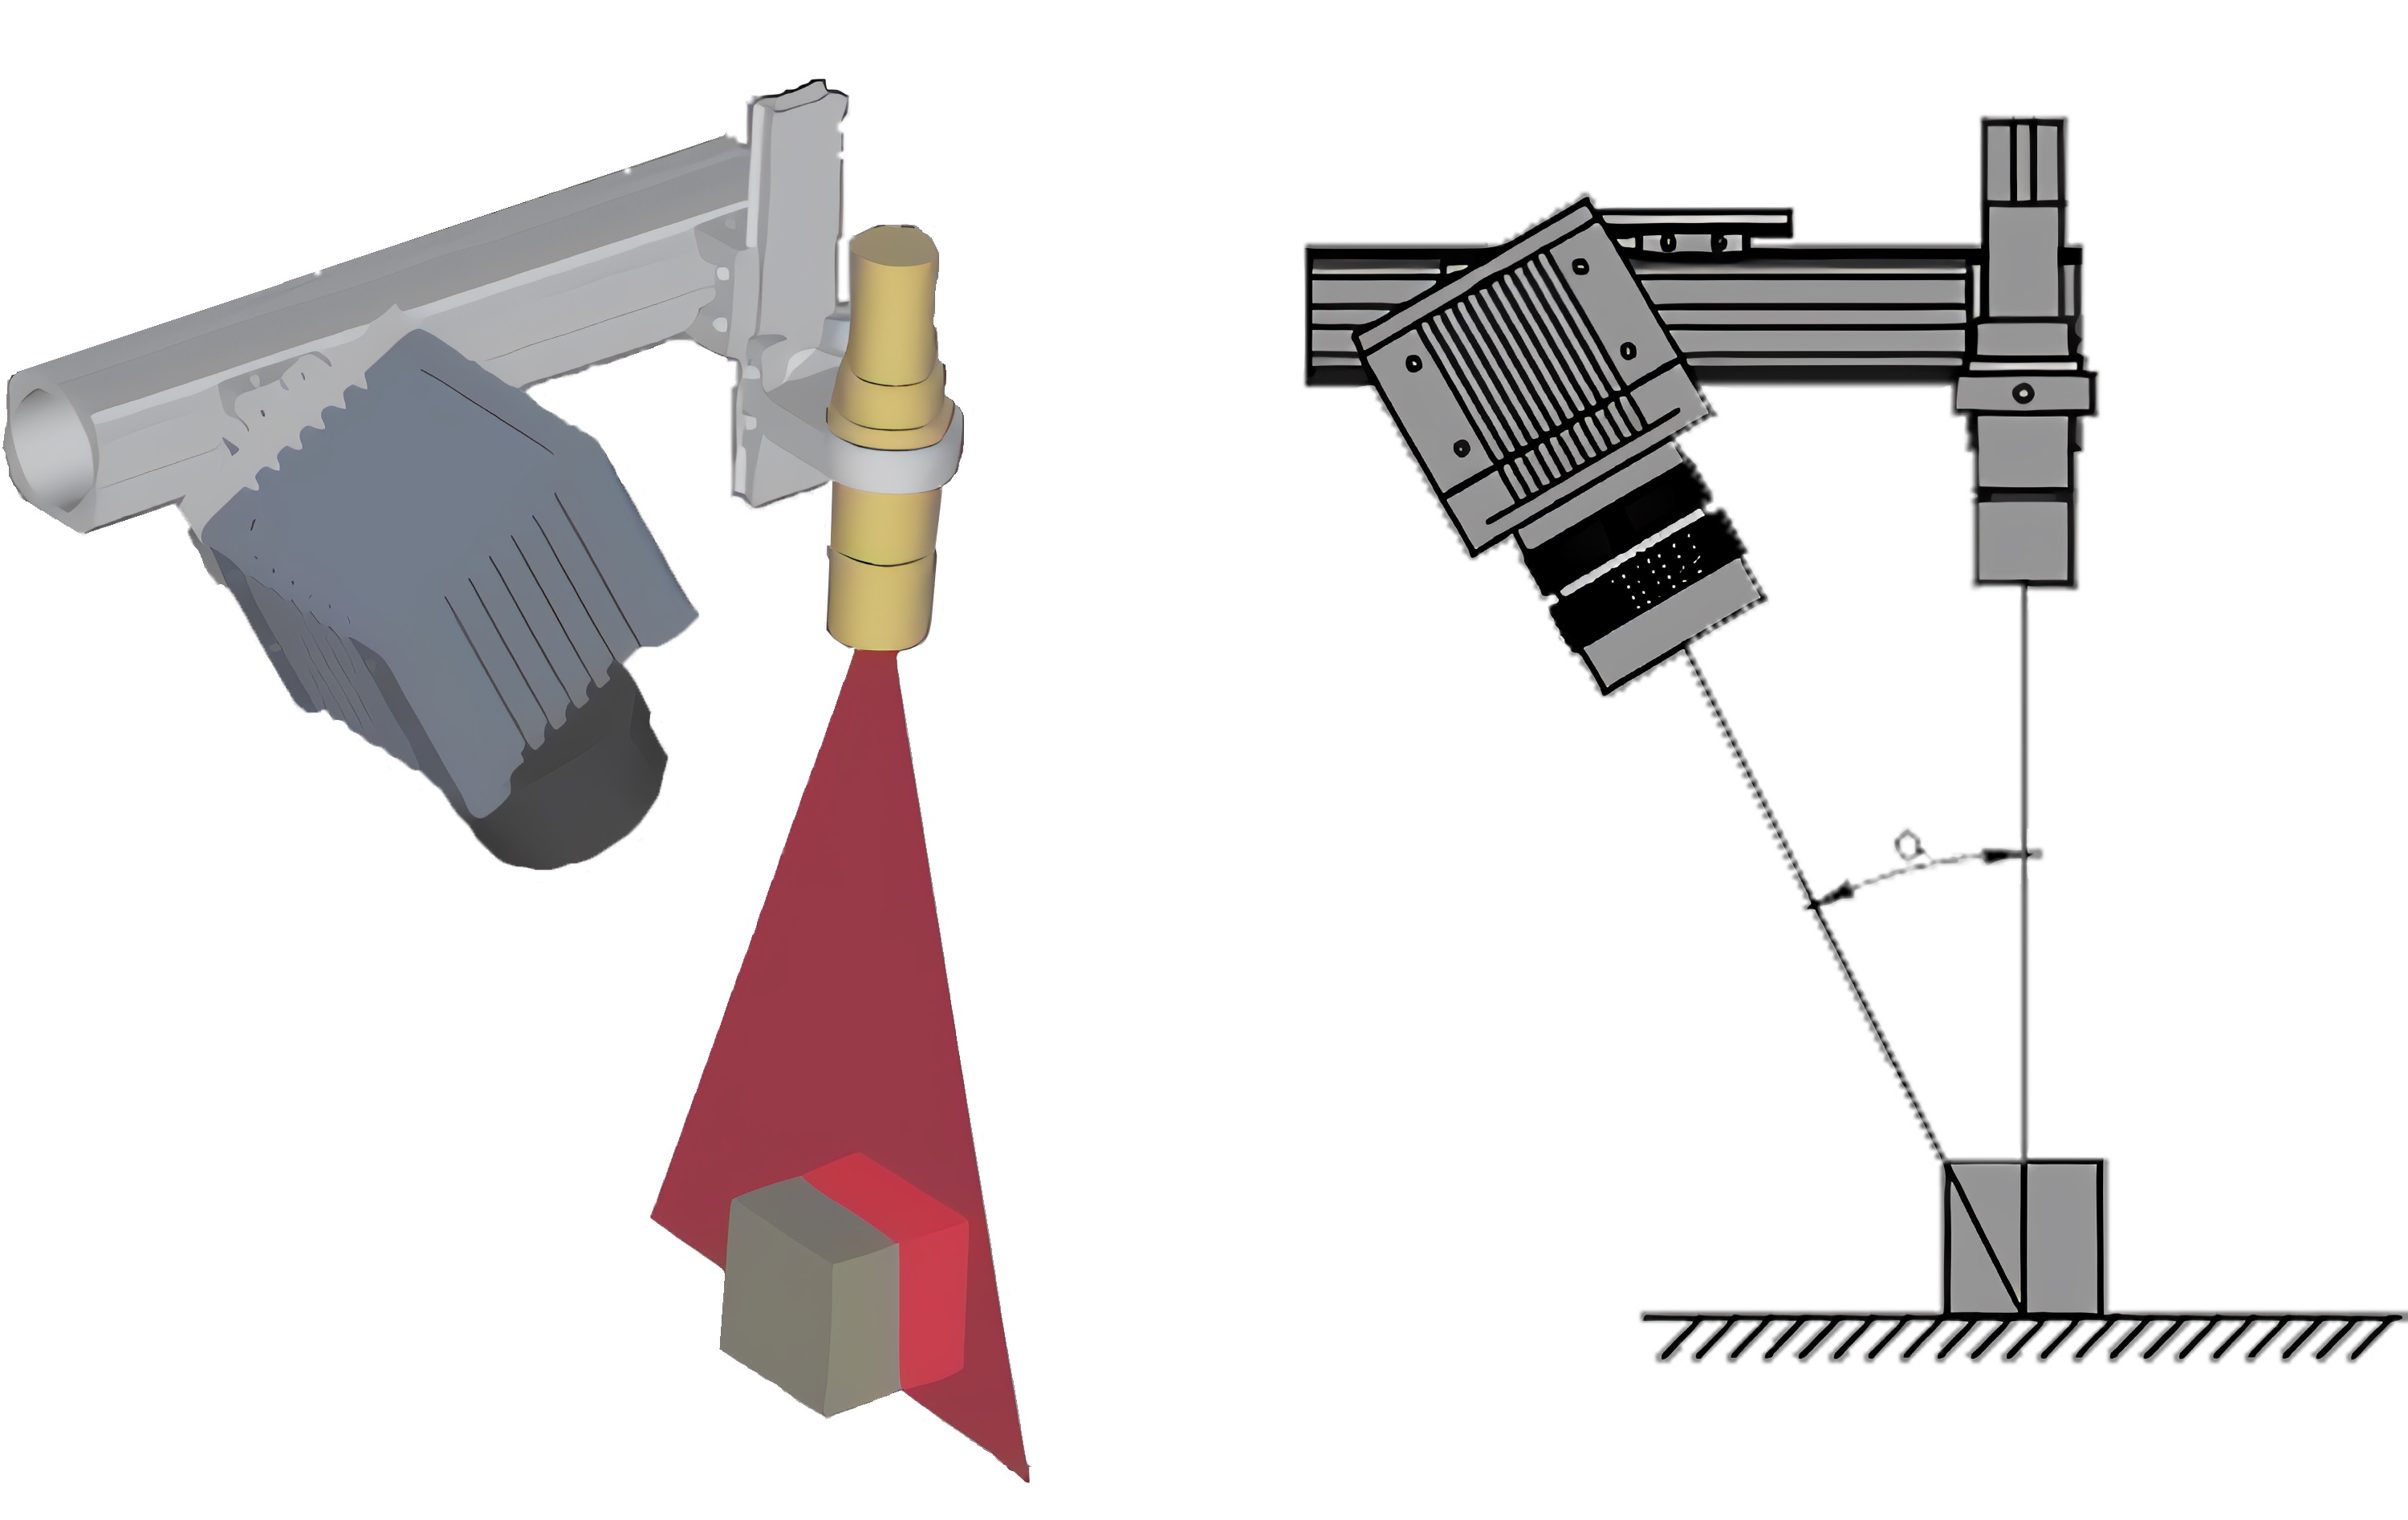
\includegraphics[width=0.8\textwidth]{laser_line_setup_upscaled_nn.jpg}
    \caption{3D laser line scanning setup \cite{method_presentation}}
    \label{fig:laser_line_setup}
\end{figure}


The captured pixel data is then processed on an FPGA to generate 3D profile data. In order to do this, the laser line, as seen by the camera, must be extracted from the pixel data. For this purpose, several methods have been proposed to extract the line data from the captured image. One of these methods employs an FIR filter to calculate the derivative of the incoming pixel stream orthogonally to the laser line direction. Afterwards, the zero crossing of this derivative is detected. The position of the zero crossing marks the position of the laser line in the camera image. From this position, the distance of the laser scanner to the scanned object can be derived.


\section{The proposed solution}


\begin{figure}[h]
    \centering
    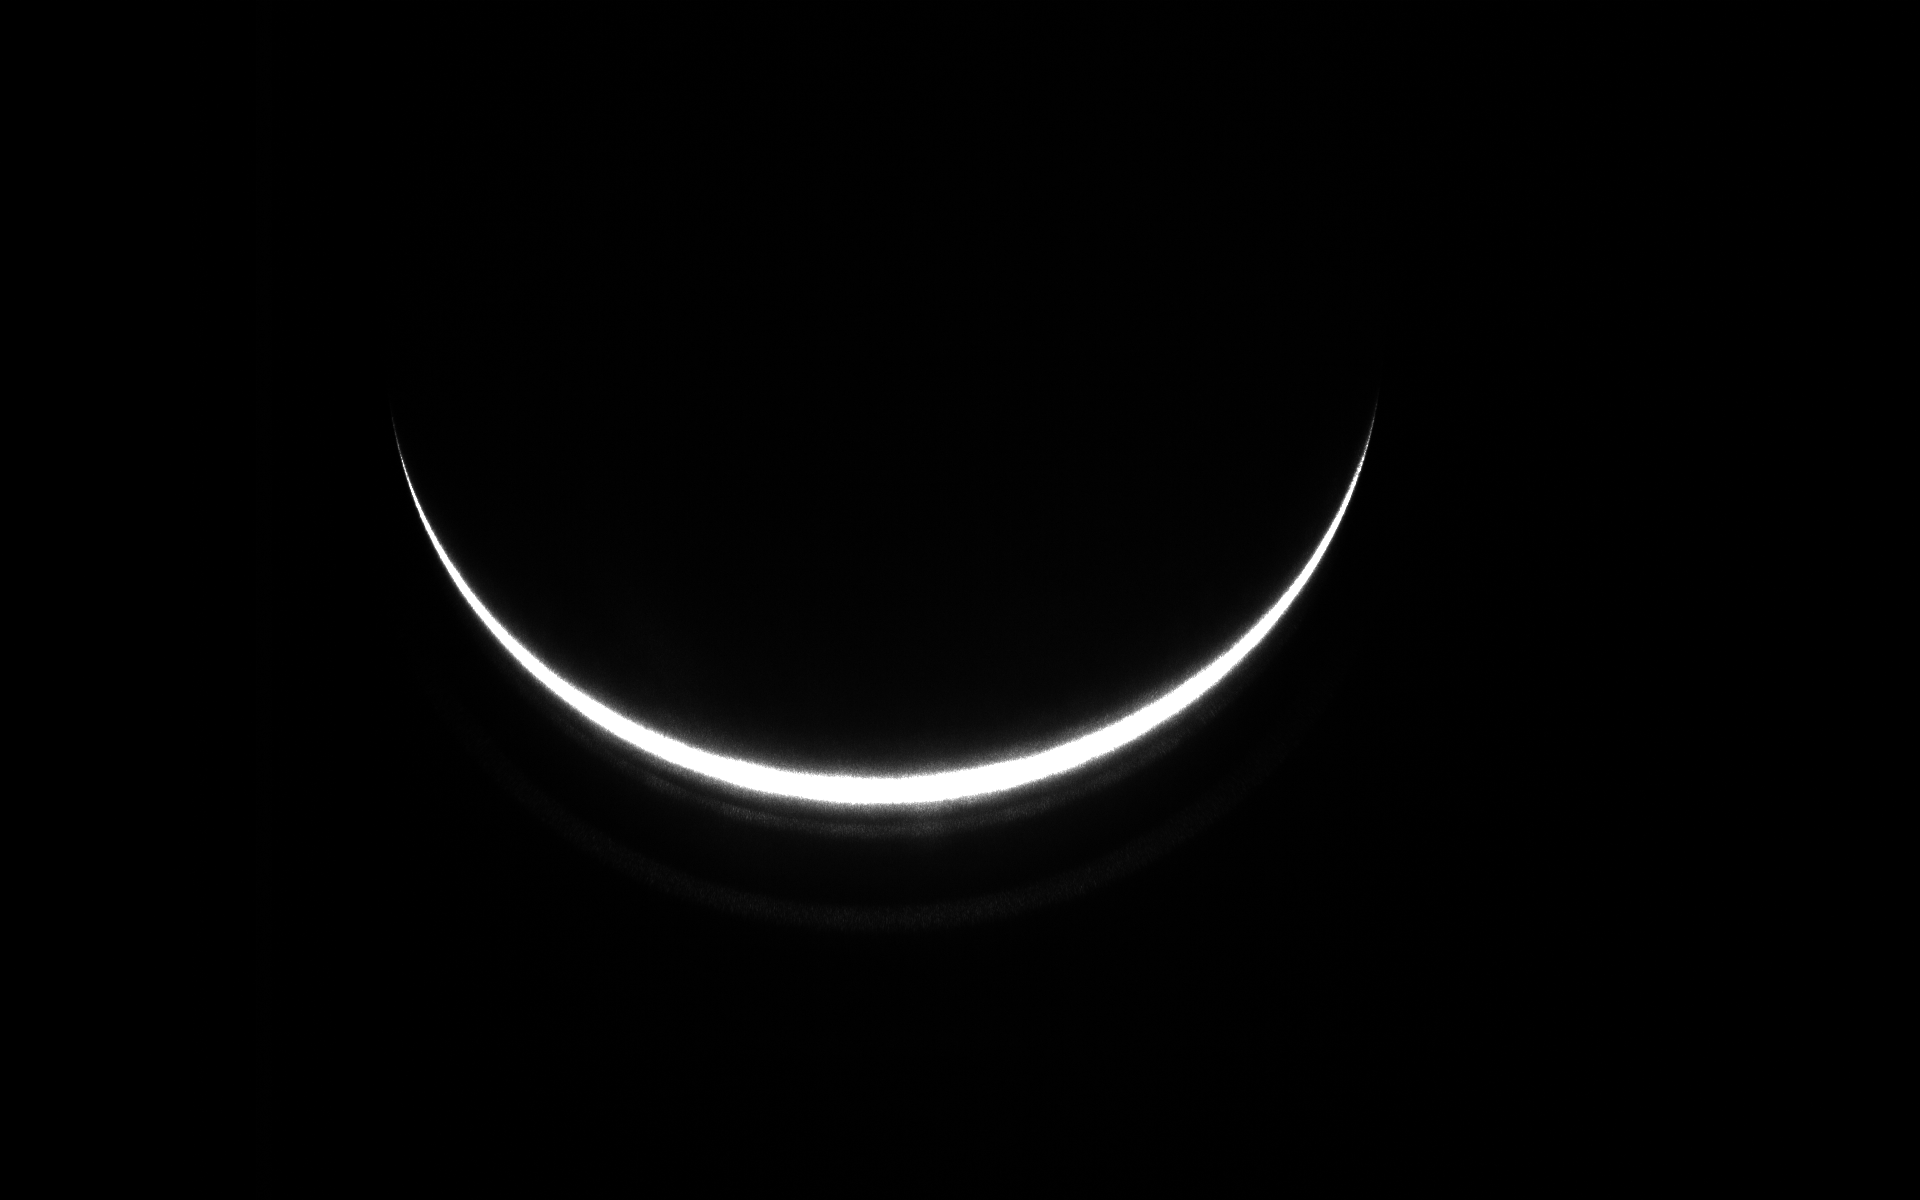
\includegraphics[width=0.8\textwidth]{sphere_laser_line.png}
    \caption{Pixel data of a laser line projected onto a spherical object}
    \label{fig:sphere_laser_line}
\end{figure}


Figure \ref{fig:sphere_laser_line} shows pixel data of a laser line cast onto a spherical shaped object. As shown in the image, the reflected laser line from the scanned object is shown as a white line in the pixel data.

The goal in this project is to extract the white line from the pixel data, and the proposed method is to process each vertical pixel line individually as shown in Figure \ref{fig:sphere_laser_line_pixel_column}. The extracted data is orthogonal to the laser line. The column data forms a gaussian distribution curve where the point of maximum intensity should point to the middle of the white laser line.


\begin{figure}[h]
    \centering
    \includesvg[width=1\textwidth]{sphere_laser_line_column.svg}
    \caption{Pixel column distribution}
    \label{fig:sphere_laser_line_pixel_column}
\end{figure}

There are several methods of exctracting the point of maximum intensity from a gaussian distribution curve. Figure \ref{fig:extraction_methods}  shows an overview of three maximum point finding methods \cite{method_presentation}. The first method is looking for the point of maximum intensity of the incoming data. Second method is to accept any point with an intensity higher than a preset threshold. Afterwars, the center position between these points is selected \cite{7794138}. Third method is to find the center of gravity of the area under the Gaussian curve \cite{7794138}. In this project, a fourth method is explored, where the derivative of the gaussian curve formed by the pixel intensity is taken. A zero-crossing in the first derivative occurs at the same position of the extremum of the incoming pixel data.


\begin{figure}[h]
    \centering
    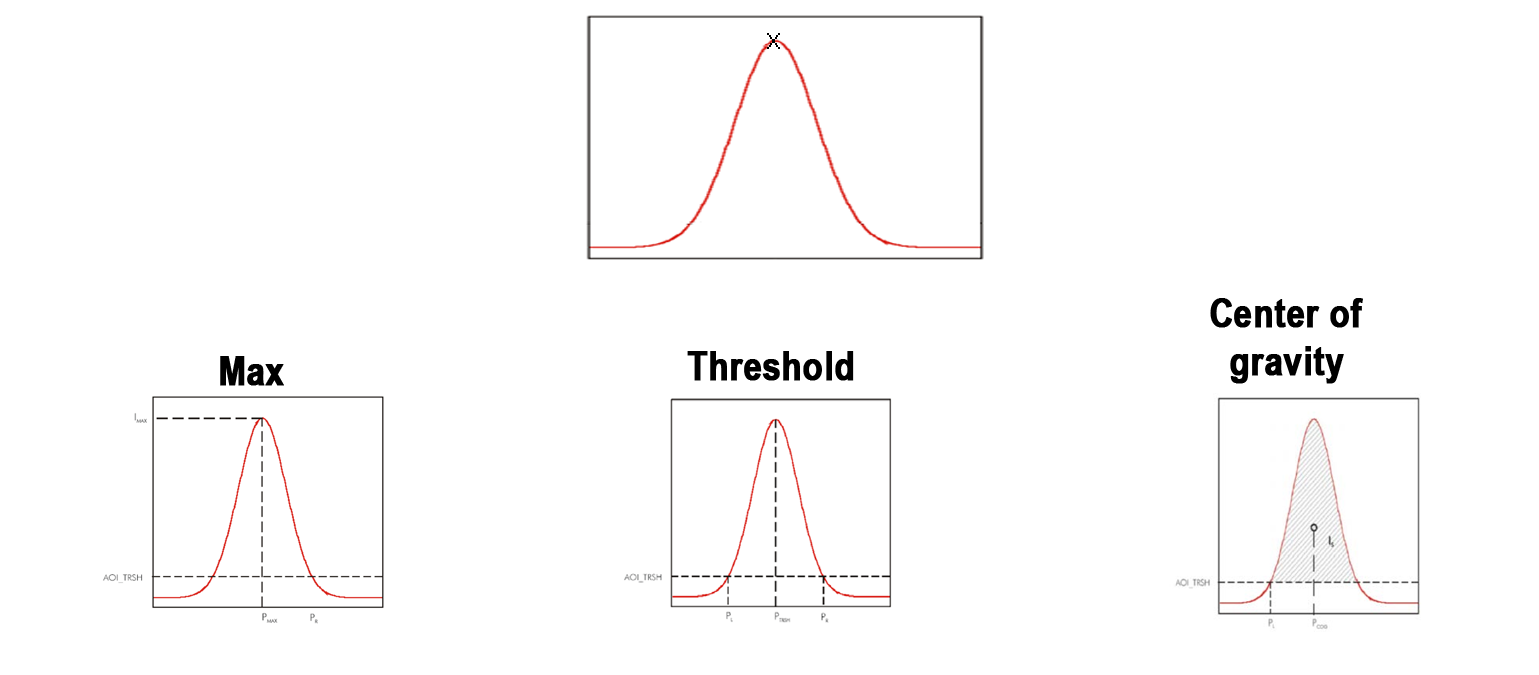
\includegraphics[width=1\textwidth]{extraction_methods.png}
    \caption{Extraction methods \cite{method_presentation}}
    \label{fig:extraction_methods}
\end{figure}

Figure \ref{fig:diff_flow} shows how the gaussian distribution curve would look like after taking its first derivative. The resulting differentiated dataset crosses from a positive value to a negative value at the point of maximum intensity. %In the example shown in \ref{fig:diff_flow} the differentiated data stagnates around zero for a bit then becomes negative because the image had a high exposure time which made the laser line over saturated.


\begin{figure}[h]
    \centering
    \includesvg[width=1\textwidth]{data_to_diff_flow.svg}
    \caption{Image data to differentiated data}
    \label{fig:diff_flow}
\end{figure}


The processing system is composed of two main parts: The filters and the zero-crossing detector. The filtering part of the system has two jobs: it needs to smooth out the data and to differentiate the gaussian curve. While the zero-crossing part of the system will detect a positive to negative going zero-crossing position, this would mark the position of the laser line in the received pixel column.




\subsection{FIR filters}

Several filter setups has been experimented with during the initial system development phase. The FIR filter setup that was implemented in VHDL in this project consists of two FIR filters, a smoothing filter and a differentiation filter. Both filters are 5 taps Savitzky–Golay filters.

The filter sizes were chosen to limit the resource usage in the final design, as increasing the number of taps didn't provide enough extra smoothing to justify the extra FPGA area needed to implement it as shown in Figure \ref{fig:smoothing_filter_tap_cmp}


\begin{figure}[h]
    \centering
    \includesvg[width=1\textwidth]{smoothing_ex_1.svg}
    \caption{Smoothing filter tap comparison}
    \label{fig:smoothing_filter_tap_cmp}
\end{figure}


The differentiation filter is a 5-tap first order Savitzky–Golay filter. Figure \ref{fig:data_through_filters} shows how the data looks like after passing both filters, as shown in the third sub-plot there is a zero-crossing at the point of maximum intensity shown in the first and second subplots.

\begin{figure}[h]
    \centering
    \includesvg[width=0.8\textwidth]{data_through_filters.svg}
    \caption{(a) Raw pixel data, (b) Smoothing filter output, (c) Differentiation filter output}
    \label{fig:data_through_filters}
\end{figure}

Since pixel data is 8-bits wide and the current system does operations on signed 16-bit integers then there was no need for normalization for filter results. The filter coefficients are as shown in \eqref{fil_coeff}:

\begin{equation}\label{fil_coeff}
    \begin{aligned}
        smoothing filter \Leftarrow \{ -3, 12, 17, 12, -3 \} \\
        differentiation filter \Leftarrow \{ 2, 1, 0, -1, -2 \}
    \end{aligned}
\end{equation}



\subsection{Zero crossing}

There are several methods to find the position at which a positive-to-negative going zero-crossing has happened. One method is to search for the pattern $\{ positive, 0, negative\} $, but the issue with this approach is that oftentimes the pixel data platues at the max value for several pixels before going down again which results in an extended amount of zeros at the zero-crossing as shown in Figure \ref{fig:zero_crossing_extended_zeros}

\begin{figure}[h]
    \centering
    \includesvg[width=0.7\textwidth]{zero_crossing_extended_zeros.svg}
    \caption{Several zero values at the zero-crossing position}
    \label{fig:zero_crossing_extended_zeros}
\end{figure}

A solution to this problem would be supporting varrying numbers of zeros in the middle of the matching pattern. This solution is not robust for an FPGA application as it requires going through the same set of data multiple times.

Another method to detect zero-crossings is to find the maximum value and the minimum value, ensure that the max value's index is less than the min value's index, then find the index in the middle. Generally this method provides accurate results for images that aren't very noisy.


\begin{figure}[h]
    \centering
    \includesvg[width=0.9\textwidth]{zero_crossing_midpoint.svg}
    \caption{Zero-crossing at midpoint of two peaks}
    \label{fig:zero_crossing_midpoint}
\end{figure}

Figure \ref{fig:zero_crossing_midpoint} shows how the zero-crossing can be located using the midpoint between the two peaks. Eq.\eqref{zero_index_eq} shows the equation used to find the zero-crossing index. $Max_i$ and $Min_i$ are the indicies of the maximum and minimum values in the dataset respectively.

\begin{equation}\label{zero_index_eq}
    Zero_i = Max_i + \frac{Min_i-Max_i}{2}
\end{equation}